\tikzset{every picture/.style={line width=0.75pt}} %set default line width to 0.75pt        

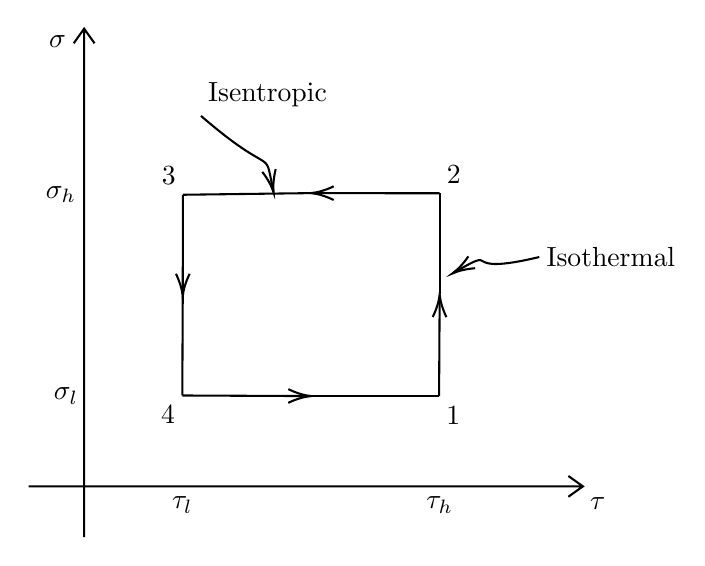
\begin{tikzpicture}[x=0.75pt,y=0.75pt,yscale=-1,xscale=1]
%uncomment if require: \path (0,444); %set diagram left start at 0, and has height of 444

%Shape: Axis 2D [id:dp10954316571485312] 
\draw  (187,247.5) -- (454,247.5)(213.7,27) -- (213.7,272) (447,242.5) -- (454,247.5) -- (447,252.5) (208.7,34) -- (213.7,27) -- (218.7,34)  ;
%Straight Lines [id:da7999053334568755] 
\draw    (384.71,204) -- (323,204) ;
%Straight Lines [id:da13773346411982845] 
\draw    (323,106.21) -- (261.29,107) ;
%Straight Lines [id:da8523825279579194] 
\draw    (261.21,156) -- (261,203.71) ;
%Straight Lines [id:da4522719625803868] 
\draw    (385,106.29) -- (385,155) ;
%Straight Lines [id:da29051283788172455] 
\draw    (261,203.71) -- (321,203.99) ;
\draw [shift={(323,204)}, rotate = 180.27] [color={rgb, 255:red, 0; green, 0; blue, 0 }  ][line width=0.75]    (10.93,-3.29) .. controls (6.95,-1.4) and (3.31,-0.3) .. (0,0) .. controls (3.31,0.3) and (6.95,1.4) .. (10.93,3.29)   ;
%Straight Lines [id:da018604575364712606] 
\draw    (385,106.29) -- (325,106.21) ;
\draw [shift={(323,106.21)}, rotate = 0.08] [color={rgb, 255:red, 0; green, 0; blue, 0 }  ][line width=0.75]    (10.93,-3.29) .. controls (6.95,-1.4) and (3.31,-0.3) .. (0,0) .. controls (3.31,0.3) and (6.95,1.4) .. (10.93,3.29)   ;
%Straight Lines [id:da43684644224945157] 
\draw    (384.71,204) -- (384.99,157) ;
\draw [shift={(385,155)}, rotate = 90.34] [color={rgb, 255:red, 0; green, 0; blue, 0 }  ][line width=0.75]    (10.93,-3.29) .. controls (6.95,-1.4) and (3.31,-0.3) .. (0,0) .. controls (3.31,0.3) and (6.95,1.4) .. (10.93,3.29)   ;
%Straight Lines [id:da05049902073104695] 
\draw    (261.29,107) -- (261.21,154) ;
\draw [shift={(261.21,156)}, rotate = 270.1] [color={rgb, 255:red, 0; green, 0; blue, 0 }  ][line width=0.75]    (10.93,-3.29) .. controls (6.95,-1.4) and (3.31,-0.3) .. (0,0) .. controls (3.31,0.3) and (6.95,1.4) .. (10.93,3.29)   ;
%Curve Lines [id:da7428626232053208] 
\draw    (433,137) .. controls (391.84,146.8) and (415.99,130.67) .. (392.5,144.14) ;
\draw [shift={(391,145)}, rotate = 330.02] [color={rgb, 255:red, 0; green, 0; blue, 0 }  ][line width=0.75]    (10.93,-3.29) .. controls (6.95,-1.4) and (3.31,-0.3) .. (0,0) .. controls (3.31,0.3) and (6.95,1.4) .. (10.93,3.29)   ;
%Curve Lines [id:da2554122965503123] 
\draw    (270,69) .. controls (306.08,100.2) and (300.32,82.92) .. (304.65,104.28) ;
\draw [shift={(305,106)}, rotate = 258.23] [color={rgb, 255:red, 0; green, 0; blue, 0 }  ][line width=0.75]    (10.93,-3.29) .. controls (6.95,-1.4) and (3.31,-0.3) .. (0,0) .. controls (3.31,0.3) and (6.95,1.4) .. (10.93,3.29)   ;

% Text Node
\draw (206.44,37.6) node [anchor=south east] [inner sep=0.75pt]    {$\sigma $};
% Text Node
\draw (456,251.4) node [anchor=north west][inner sep=0.75pt]    {$\tau $};
% Text Node
\draw (211.29,107) node [anchor=east] [inner sep=0.75pt]    {$\sigma _{h}$};
% Text Node
\draw (212.29,204) node [anchor=east] [inner sep=0.75pt]    {$\sigma _{l}$};
% Text Node
\draw (261,251.11) node [anchor=north] [inner sep=0.75pt]    {$\tau _{l}$};
% Text Node
\draw (385,251.11) node [anchor=north] [inner sep=0.75pt]    {$\tau _{h}$};
% Text Node
\draw (435,137) node [anchor=west] [inner sep=0.75pt]   [align=left] {Isothermal};
% Text Node
\draw (272,66) node [anchor=south west] [inner sep=0.75pt]   [align=left] {Isentropic};
% Text Node
\draw (386.71,207.4) node [anchor=north west][inner sep=0.75pt]    {$1$};
% Text Node
\draw (387,102.89) node [anchor=south west] [inner sep=0.75pt]    {$2$};
% Text Node
\draw (259.29,103.6) node [anchor=south east] [inner sep=0.75pt]    {$3$};
% Text Node
\draw (259,207.11) node [anchor=north east] [inner sep=0.75pt]    {$4$};


\end{tikzpicture}
